
\begin{figure}[t!]
    \centering
    \begin{subfigure}[t]{0.32\textwidth}
        \vspace{0pt}
        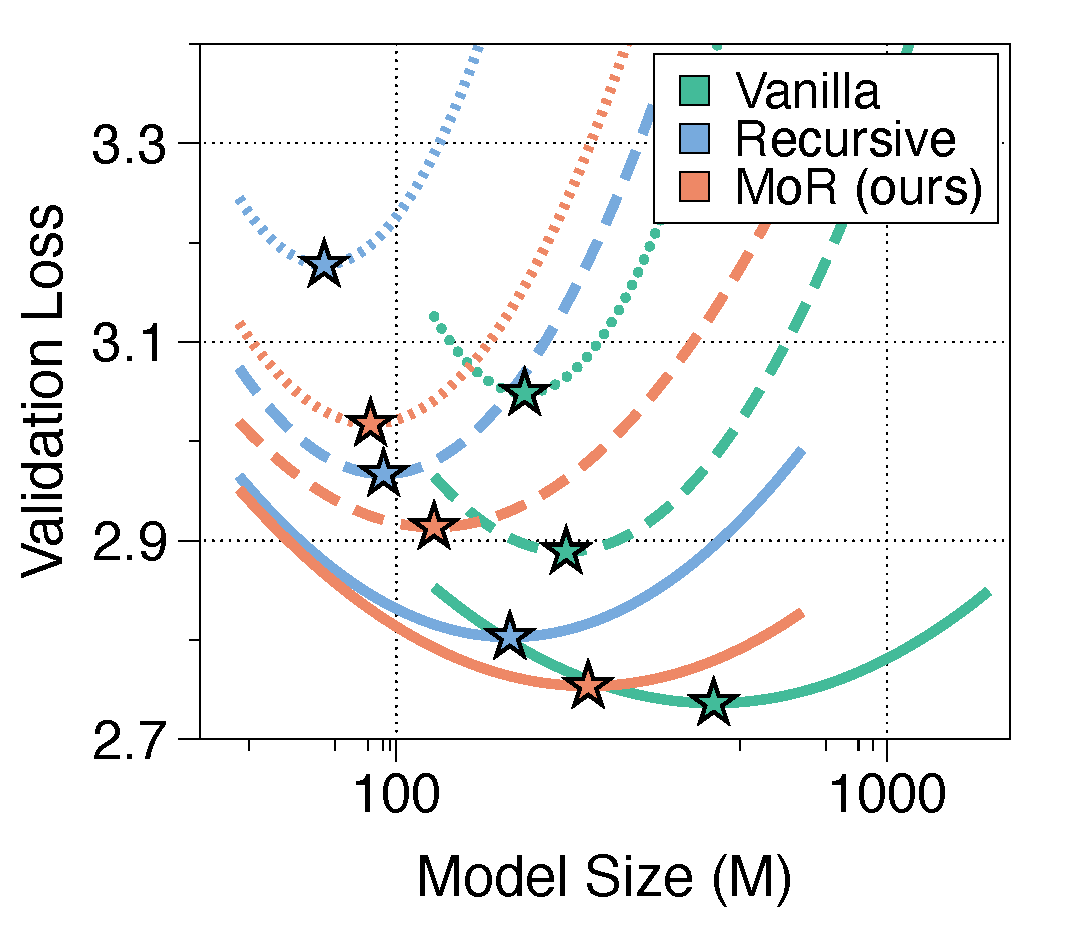
\includegraphics[width=\textwidth]{figs/scaling_laws/scaling_law_one_figure.pdf}
            \captionsetup{justification=centering}
        \subcaption{Compute-optimal scaling}
        \label{fig:isoflops_qualitative-a}
    \end{subfigure}
    \hfill
    \begin{subfigure}[t]{0.385\textwidth}
        \vspace{-4pt}
        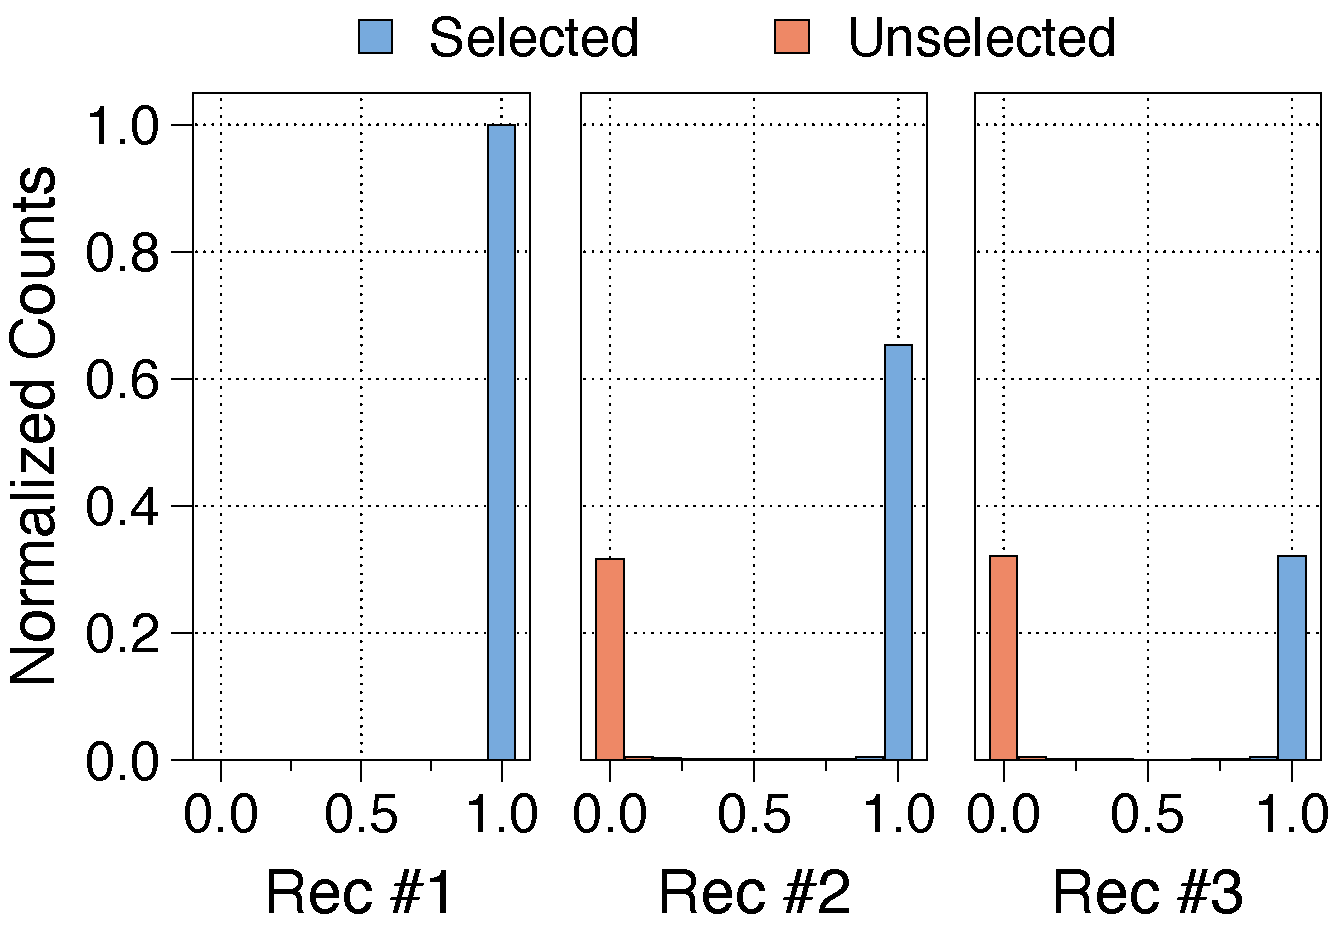
\includegraphics[width=\textwidth]{figs/weight_values/weight_values.pdf}
        \vspace{-4pt}
            \captionsetup{justification=centering}
        \subcaption{Learned router scores}
        \label{fig:isoflops_qualitative-b}
    \end{subfigure}
    \hfill
    \begin{subfigure}[t]{0.275\textwidth}
        \vspace{0pt}
        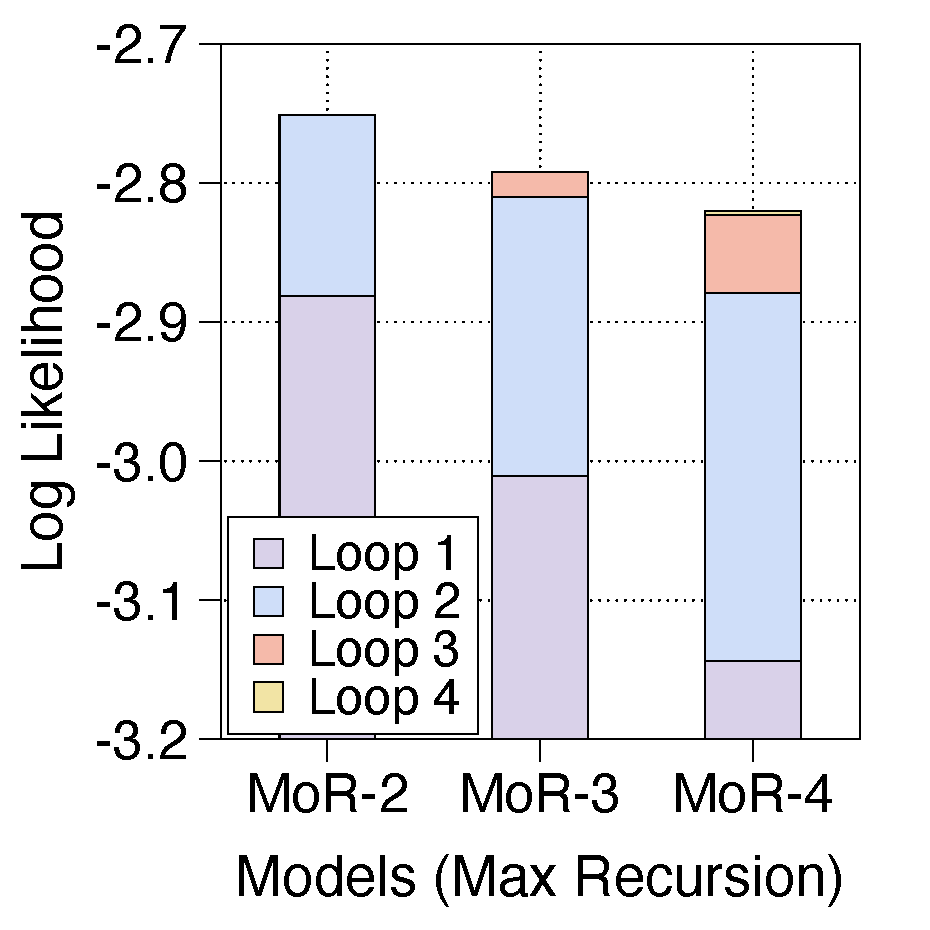
\includegraphics[width=\textwidth]{figs/test_time_scale/test_time_scale.pdf}
            \captionsetup{justification=centering}
        \subcaption{Test-time scaling}
        \label{fig:isoflops_qualitative-c}
    \end{subfigure}
    \caption{
    (a) Compute-optimal scaling analysis for three model architectures. Each star indicates the optimal model size for a given compute budget. We visualize the results in \S\ref{subsec:scaling_laws} by fitting polynomial functions for each architecture and FLOPs budget, and derive the optimal points from these fits. (b) Distribution of router outputs for selected and unselected tokens at each recursion step. As an example, a 360M size-based MoR model with $N_r=3$, expert-choice router with auxiliary loss, and recursion-wise caching, is used. (c) Test-time scaling analysis illustrating the cumulative log-likelihood improvement with increasing recursion depth, measured over 500 samples. As we increase $N_r$ based on a 360M model size, the number of unique parameters in MoR decreases, resulting in a gradual decline in overall performance (i.e., a decrease in log-likelihood). All models are trained by an expert-choice router with auxiliary loss and a recursion-wise caching mechanism.\looseness=-1
    }    
    \label{fig:isoflops_qualitative}
\end{figure}